\documentclass[10 pt,usenames,dvipsnames, oneside]{article}
\usepackage{../../../modelo-ensino-medio}



\begin{document}

\begin{center}
  \begin{minipage}[l]{3cm}
\includegraphics[width=2cm]{logo}    
\end{minipage}\hfill
\begin{minipage}[r]{.8\textwidth}
 {\Large \scshape Atividade: }  
\end{minipage}
\end{center}
\vspace{.2cm}

\ifdefined\prof
\begin{objetivos}
\item \phantom{a}
\end{objetivos}

\begin{goals}
\begin{enumerate}

\item Interpretar uma situação que envolve movimento retilíneo uniforme a partir do gráfico que representa a relação entre distância e tempo.
\item Compreender o modelo de variação que se estabelece entre as variáveis distância e tempo.
\item Constatar que a distância percorrida sempre será a mesma em intervalos de tempo iguais.
\item Identificar que mesmo a taxa de variação sendo constante, as grandezas envolvidas não são proporcionais.
\end{enumerate}


\tcblower


\begin{itemize}
\item Já no item a) é comum boa parte dos alunos não identificarem a posição do ponto de referência, principalmente por criar associações equivocadas entre o gráfico e a situação real. Para isso utilize algum modelo que deixe claro que a reta apresentada do gráfico não é o “caminho” percorrido pela pessoa. Por exemplo:

\begin{figure}[H]
\centering

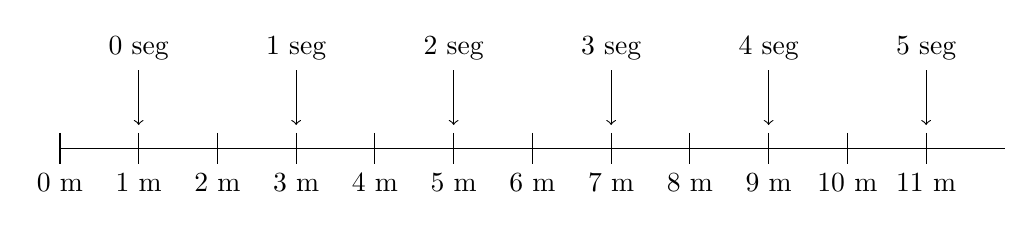
\begin{tikzpicture}
\draw (0,0) -- (12,0);
\foreach \x/\y/\z in {0/1/0,2/3/1,4/5/2,6/7/3,8/9/4,10/11/5}{
	\draw (\x,.2) -- (\x,-.2);
1	\draw (\y,.2) -- (\y,-.2);
	\node [below] at (\x,-.2) {$\x$ m};
	\node [below] at (\y,-.2) {$\y$ m};
	\draw [<-] (\y,.3) -- (\y,1) node [above] {$\z$ seg};
	
}
\end{tikzpicture}
\end{figure}

\item Recomendamos que, se possível, discuta com seus alunos uma variante do problema. O caso em que, mesmo que a pessoa não ande em linha reta, o gráfico continua representando a relação entre a distância percorrida e o tempo de percurso. Apresente por exemplo percursos diferentes, refazendo as perguntas, como por exemplo:

\begin{figure}[H]
\centering
\usetikzlibrary{arrows.meta}


\begin{tikzpicture}[scale=.75]
\draw circle (2cm);
\node at (0:2) {$\times$} node at (0:2) [right, overlay] {Ponto de partida}; 
\node at (300:2) {$\times$} node at (300:2) [below right, overlay] {Ponto de referência}; 

\draw [-{>[length=2mm,width=3mm]},  samples=1000] (2,0) arc (0:30:2);
\draw [-{>[length=2mm,width=3mm]}, samples=1000] (2,0) arc (0:60:2);

\begin{scope}[scale=2,shift={(3.5,.25)}]
\draw (0,0) -- (2,0) -- (.2,-1) -- (-.2,-.2);
\node at (0,0) {$\times$};
\node [above] at (0,0) {Ponto de referência};
\node at (2,0) {$\times$};
\node [right,] at (2,0) {Ponto de partida};
\end{scope}
\end{tikzpicture}

\end{figure}


\item Discuta com seus alunos o motivo da função não ser linear e consequentemente, nesta situação, a relação entre as grandezas não ser proporcional. Utilize o fato de não atender o Teorema Fundamental da Proporcionalidade.

\item Caso seus alunos já tenham estudado esse conteúdo em Física, aproveite para relacionar a função $f(t)=at+b$ com a equação tradicional do Movimento Uniforme: $S=S+Vt$, associando S com $f(t)$ ; $S_0$ com $b$ e $V$ com $a$.
 
\end{itemize}
\end{goals}

\bigskip
\begin{center}
{\large \scshape Atividade}
\end{center}
\fi

O gráfico a seguir mostra a variação da distância a um ponto de referência de uma pessoa que caminha em linha reta durante \(4\) segundos. Algumas informações sobre o movimento podem ser extraídas diretamente dessa representação gráfica.
\phantomsection\label{\detokenize{AF107-4:fig-tempo-distancia}}
\begin{figure}[H]
\centering

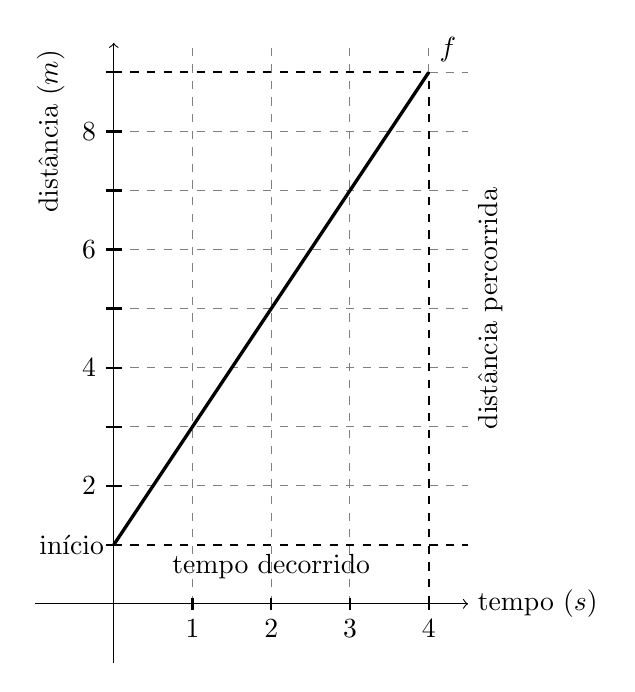
\begin{tikzpicture}[yscale=.75]

\draw [dashed, help lines, thin] (0,0) grid (4.5,9.5);
\draw [->] (-1,0) -- (4.5,0);
\draw [->] (0,-1) -- (0,9.5);

\draw [\currentcolor, very thick] (0,1) -- (4,9) node [above right, black] {$f$};
\draw [thick, dashed] (0,1) -- (4.5,1);
\draw [thick, dashed] (4,0) -- (4,9);
\draw [thick, dashed] (0,9) -- (4,9);

\foreach \x in {1,...,4}{
\draw [ thick] (\x,-.1) -- (\x,.1);
\node [below] at (\x,-.1) {$\x$};}

\foreach \x in {2,4,...,8} \node [left] at (-.1,\x) {$\x$};
\foreach \x in {1,...,9} \draw [thick] (-.1,\x) -- (.1,\x);

\node [below] at (2,1) {tempo decorrido};
\node [left] at (0,1) {início};
\node [rotate=90, above] at (-.5,8) {distância ($m$)};
\node [rotate=90, below] at (4.5,5) {distância percorrida};
\node [right] at (4.5,0) {tempo ($s$)};
\end{tikzpicture}


\label{\detokenize{AF107-4:fig-tempo-distancia}}\end{figure}
\begin{enumerate}
\item {} 
A que distância do ponto de referência estava a pessoa no início da contagem do tempo? E ao final de \(4\) segundos?

\item {} 
Qual a distância total percorrida?

\item {} 
É possível saber se ele está se afastando ou se aproximando do ponto de referência? Como?

\item {} 
Qual a velocidade média da pessoa no intervalo de tempo de \(0\) a \(4\) segundos?

\item {} 
A que distância a pessoa estava do ponto de referência após \(1\) segundo do início da caminhada? Qual a distância percorrida por ela nesse intervalo de tempo?

\item {} 
Qual a distância percorrida pela pessoa entre \(1\) e \(2\) segundos? E entre \(3\) e \(4\) segundos?

\item {} 
O que se pode concluir, a partir das suas respostas nos itens (e) e (f), sobre a variação da distância percorrida a cada minuto de caminhada?

\item {} 
As grandezas relacionadas pelo gráfico são proporcionais? Porque?

\end{enumerate}

\ifdefined\prof
\begin{solucao}
\begin{enumerate}
\item $1$ metro. $9$ metros.
\item $8$ metros.
\item Sim, ela está se afastando. A medida que o tempo aumenta a distância até o ponto de referência também aumenta. Isto é, a função é crescente.
\item A velocidade média é $V=9−14−0=2$ m/s.
\item $3$ metros. $2$ metros.
\item $3$ metros em ambos os intervalos de tempo.
\item A cada segundo a pessoa se afasta $2$ metros do ponto de referência.
\item Não, pois a distância até o ponto de referência em $2$ segundos é $5$ metros e em $1$ segundo é $3$ metros, ou basta ver que o gráfico não passa pela origem do plano cartesiano .
\end{enumerate}
\end{solucao}
\fi

\end{document}